\documentclass{article}

\usepackage{graphicx}
\usepackage{tikz}
\usepackage{tikzsymbols}
\usetikzlibrary{calc,patterns,shapes.geometric}
\pagestyle{empty}
\usepackage[margin=0pt]{geometry}
\geometry{papersize={14in,12in}}

\def\centerarc[#1](#2)(#3:#4:#5){\draw[#1] ($(#2)+({#5*cos(#3)},{#5*sin(#3)})$) arc (#3:#4:#5);}

\begin{document}
	\begin{figure}
		\centering
		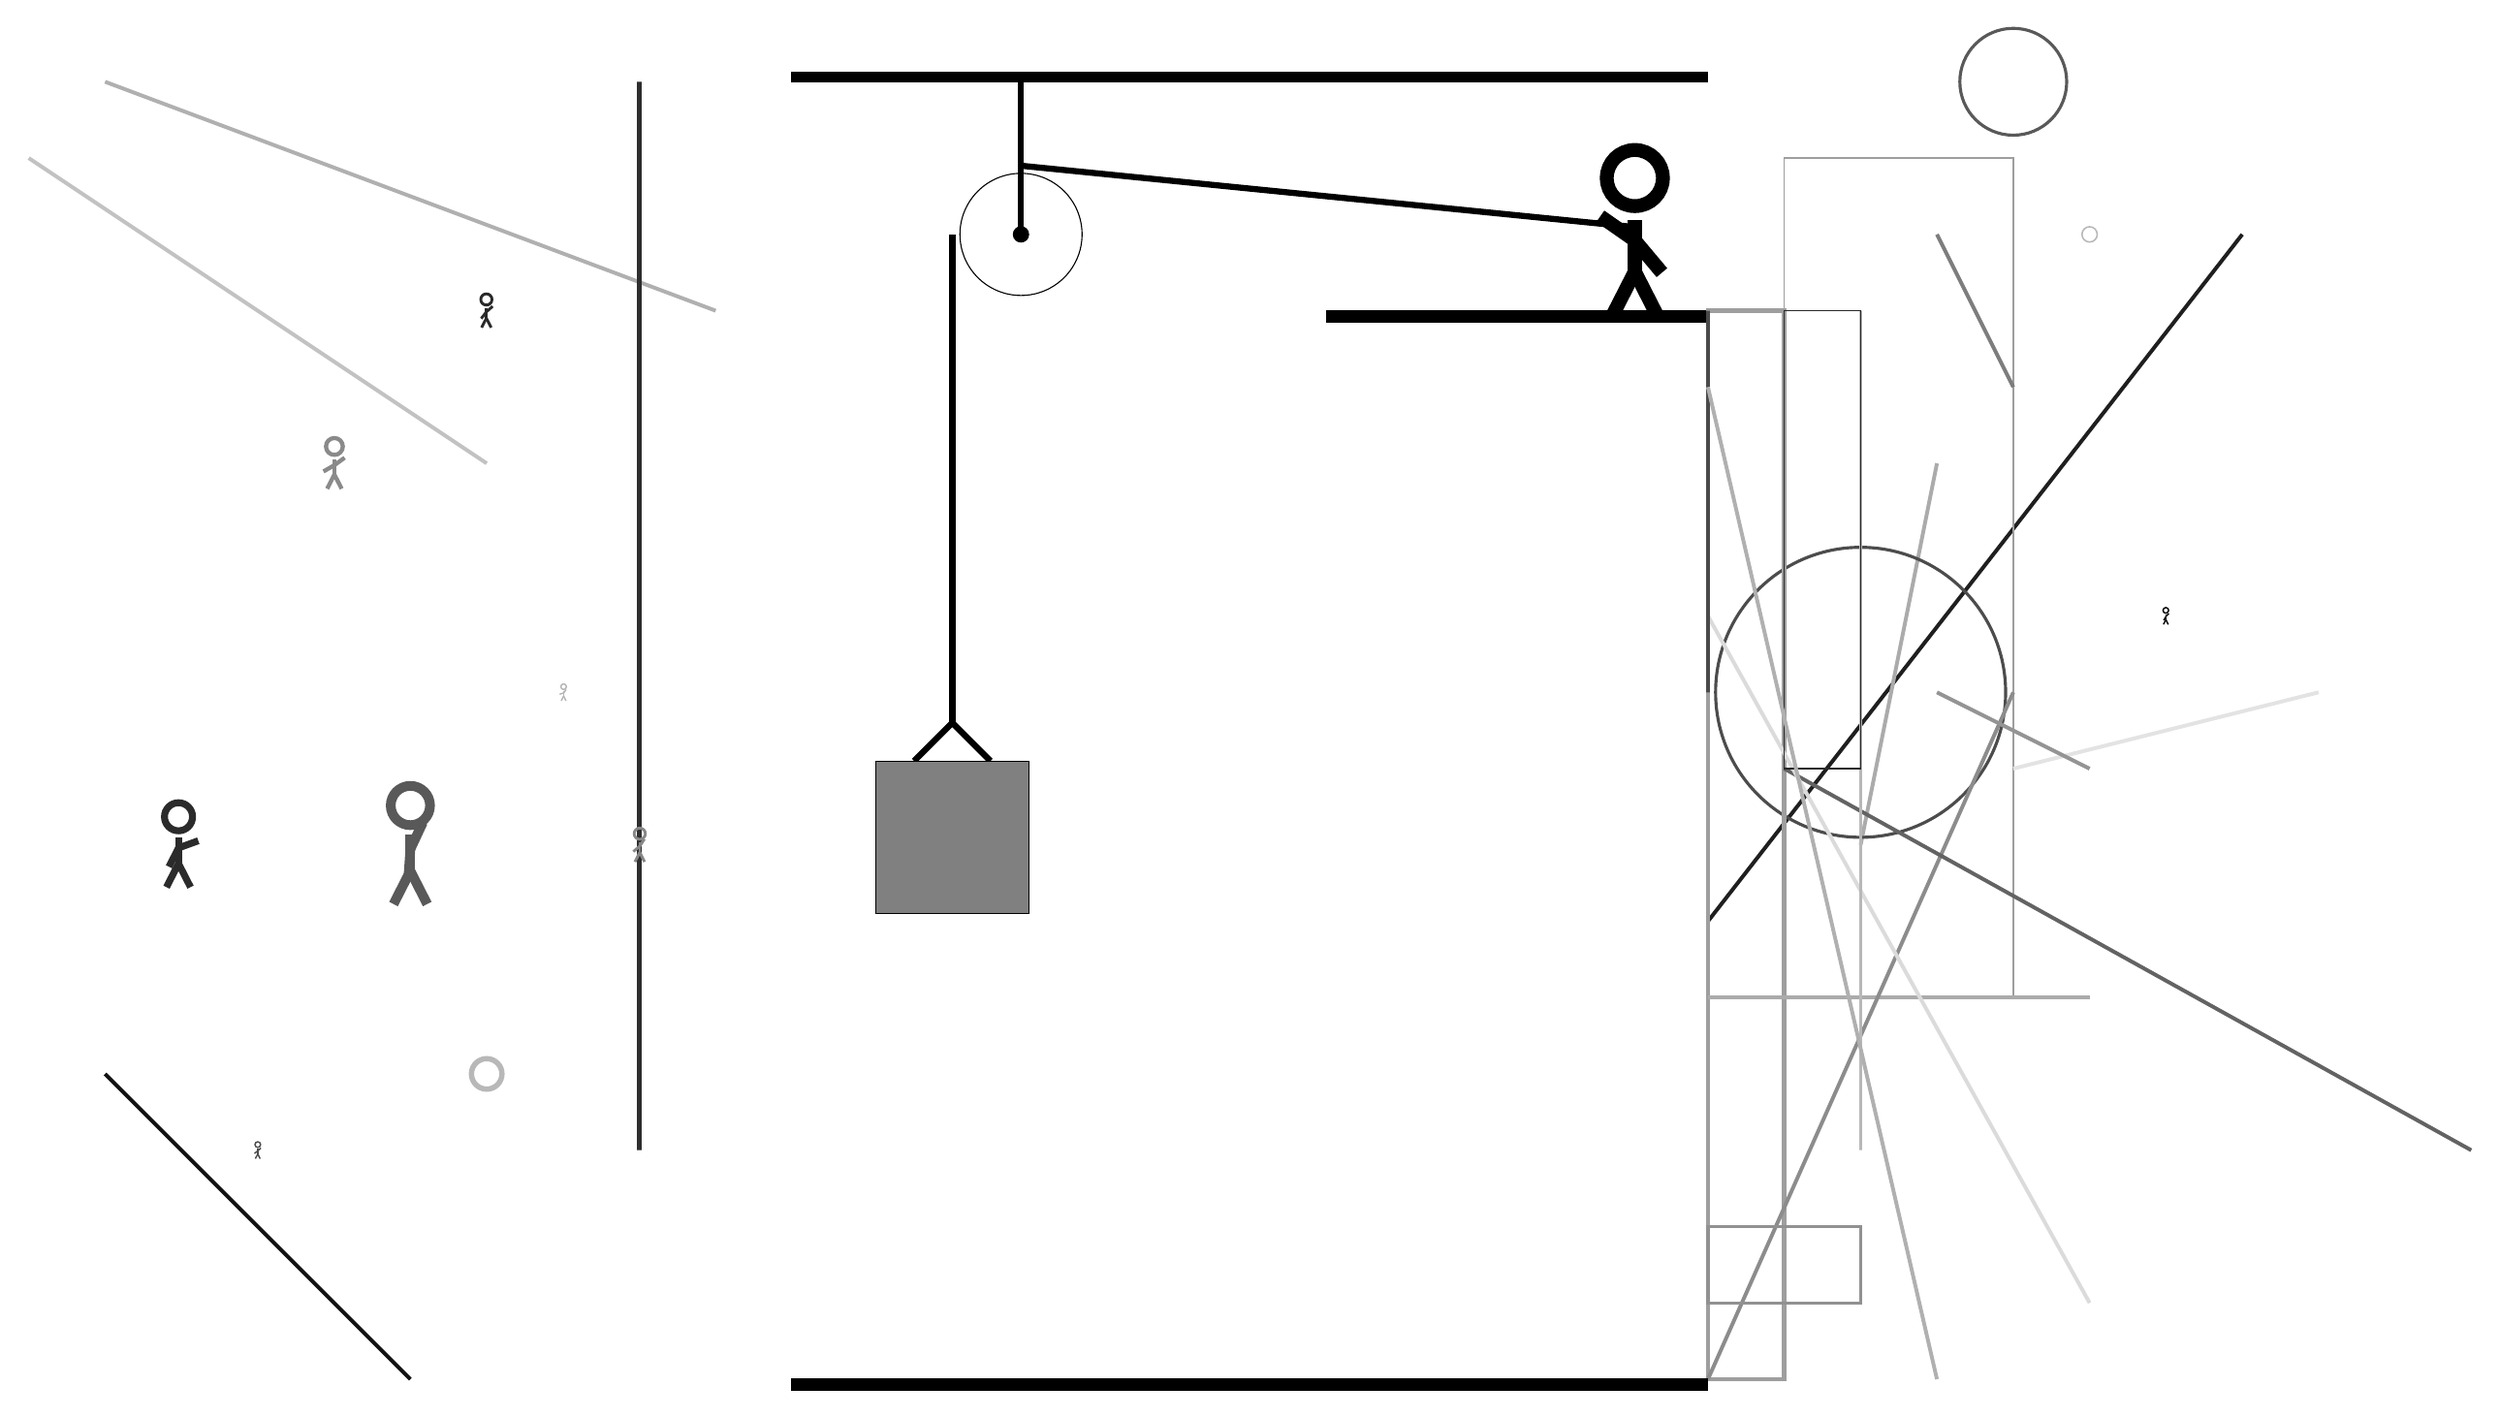
\begin{tikzpicture}
			%%%%% START %%%%%
			
			\draw[fill=black] (-2, 14) rectangle (10, 14.125);
			
			\draw (1, 12) circle (0.8);
			\draw[fill=black] (1, 12) circle (0.1);
			\draw[line width=0.8mm] (1, 14) -- (1, 12);
			
			\draw[line width=0.8mm](-0.4, 5.1) --  (0.1, 5.6) -- (0.6, 5.1);
			\draw[fill=black!50] (-0.9, 5.1) rectangle (1.1, 3.1);
			
			\draw[line width=0.8mm](0.1, 12) -- (0.1, 5.6);
			\centerarc[line width=0.8mm](1, 12)(90:180:0.9)
			\draw[line width=0.8mm](1, 12.9) -- (9, 12.1);
			
			\node at (9, 12) {\Strichmaxerl[10][-35][-50]};
			\draw[fill=black] (5, 11) rectangle (10, 10.85);
			
			\draw[line width=0.5mm, color=black!88](10, 3) -- (17, 12);
			
			\draw[line width=0.5mm, color=black!24](-6, 9) -- (-12, 13);
			\draw[line width=0.2mm, color=black!38] (11, 2) rectangle (14, 13);
			\node[line width=0.5mm, color=black!29] at (-5, 6) {\Strichmaxerl[1][18][53]};
			
			\draw[line width=0.5mm, color=black!51](14, 10) -- (13, 12);
			\draw[line width=0.5mm, color=black!33](13, 9) -- (12, 4);
			
			\draw [line width=0.4mm, color=black!70](12, 6) circle (1.9);
			
			\draw[line width=0.6mm, color=black!38] (10, 11) rectangle (11, -3);
			\draw [line width=0.7mm, color=black!28](-6, 1) circle (0.2);
			\draw[line width=0.5mm, color=black!33](10, 2) -- (15, 2);
			
			\node[line width=0.5mm, color=black!65] at (-7, 4) {\Strichmaxerl[7][86][65]};
			\draw[line width=0.5mm, color=black!45](10, -3) -- (14, 6);
			\draw[line width=0.5mm, color=black!61](11, 5) -- (20, 0);
			\node[line width=0.7mm, color=black!99] at (16, 7) {\Strichmaxerl[1][60][45]};
			\node[line width=0.4mm, color=black!70] at (-9, 0) {\Strichmaxerl[1][39][41]};
			\draw [line width=0.4mm, color=black!65](14, 14) circle (0.7);
			
			\draw[line width=0.5mm, color=black!14](15, -2) -- (10, 7);
			
			\node[line width=0.5mm, color=black!46] at (-8, 9) {\Strichmaxerl[3][30][36]};
			\draw[line width=0.6mm, color=black!71] (10, 11) rectangle (10, 6);
			
			\draw [line width=0.2mm, color=black!28](15, 12) circle (0.1);
			\draw[line width=0.5mm, color=black!93](-7, -3) -- (-11, 1);
			\draw[line width=0.5mm, color=black!31](-3, 11) -- (-11, 14);
			\draw[line width=0.4mm, color=black!28] (12, 11) rectangle (12, 0);
			\draw[line width=0.5mm, color=black!11](14, 5) -- (18, 6);
			\draw[line width=0.2mm, color=black!84] (12, 5) rectangle (11, 11);
			
			\draw[line width=0.7mm, color=black!82] (-4, 14) rectangle (-4, 0);
			
			\draw[line width=0.5mm, color=black!31](13, -3) -- (10, 10);
			\node[line width=0.3mm, color=black!84] at (-6, 11) {\Strichmaxerl[2][52][42]};
			
			\node[line width=0.4mm, color=black!47] at (-4, 4) {\Strichmaxerl[2][40][57]};
			\draw[line width=0.3mm, color=black!34] (-3, 5) rectangle (-3, 5);
			\node[line width=0.7mm, color=black!83] at (-10, 4) {\Strichmaxerl[5][63][20]};
			
			\draw[line width=0.5mm, color=black!42](15, 5) -- (13, 6);
			\draw[line width=0.4mm, color=black!43] (12, -2) rectangle (10, -1);
			
			\draw[fill=black] (-2, -3) rectangle (10, -3.15);
			
			%%%%% END %%%%%
		\end{tikzpicture}
	\end{figure}	
\end{document}